\section{Three-dimensional simulations}
In this section we briefly review 3D simulations carried 
out using ZEUS-MP and PLUTO. The main purpose is to check 
the above results with different numerical codes, and validate  
the 2D approximation.    

The 3D disc has radial size
$[r_\mathrm{min},r_\mathrm{max}]=[0.4,10]R_0$ and vertical extent 
$n_H=2$ scale-heights. The resolution is $N_r\times N_\theta\times
N_\phi=256\times32\times256$. This corresponds to about $4$ cells per
$H$in radius. 
Because of the much reduced resolution 
compared to 2D, we use a smooth perturbation by setting
$\delta = 10^{-3}$ and $M=1$ in Eq. \ref{randpert}. This corresponds
to a single $m=1$ disturbance in $R\in[R_1,R_2]$, which was found to dominate
the 2D simulation.  

Our 3D discs are initialised in approximate equilibrium only, so we
first evolve the disc without perturbations using  
$(\lmax,\mmax)=(32,0)$ up to $t=100P_0$, during which 
meridional velocities are damped out. We then restart the simulation
with the above perturbation and $(\lmax,\mmax)=(32,32)$. 


Fig. \ref{3d_ampmax} plots the amplitude of the $m=1$ spirals measured
in the ZEUS-MP and PLUTO runs. We also show results from strictly
isothermal discs ($q=0$), which clearly display no growth. %why no high m
                                %modes as in 2D for iso disc?
                                %resolution?
Results from ZEUS-MP appears to be off-set from that obtained using
PLUTO. We suspect this may be due to larger numerical noise in the
ZEUS-MP code. Thus the $m=1$ spiral grows to a larger amplitude by the
end of the run. However, we measure similar growth rates,
\begin{align*}
&\gamma \simeq 0.0073\Omega_k(R_0) \quad\quad \mathrm{PLUTO},\\
&\gamma \simeq 0.0075\Omega_k(R_0) \quad\quad \mathrm{ZEUS-MP}.
\end{align*}
Both are smaller than the 2D simulations above. This may be due to the
low resolutions adopted. 
%growth rate does not depend on pert amp

\begin{figure}
  \includegraphics[width=\linewidth]{figures/m1_analysis_plot_ampmax3d.ps}
  \caption{Evolution of the maximum $m=1$ density in  $r\in[R_1,R_2]$
    measured in the 3D simulations. Both discs with a imposed
    temperature gradient ($q=1$) and a strictly isothermal disc
    ($q=0$) are shown. 
    \label{3d_ampmax}}   
\end{figure}

Visualisations of the 3D simluations are shown in Fig. \ref{3d_prelim} for
both ZEUS-MP and PLUTO. The snapshots are chosen for when the spiral
amplitudes are similar. The agreement between the two codes, as well
as with the 2D simulations, is satisfactory. 

%but a longer PLUTO simulation was 
%needed to achieve similar mode amplitudes in ZEUS-MP. 


\begin{figure}
  \begin{center}
    \subfigure[ZEUS-MP]{
      \includegraphics[scale=0.33]{figures/polarxy_dens015_zeus}
    }
    \subfigure[PLUTO]{
      \includegraphics[scale=0.33]{figures/pdisk_020}
    }
  \end{center}
  \caption{Three-dimensional simulations using the (a) ZEUS-MP and (b)
    PLUTO. The non-axisymmetric midplane density is shown. Here $\psi
    \equiv \pi/2 - \theta$ is the angular height 
    from the midplane.\label{3d_prelim}}   
\end{figure}

\subsection{Vertical motion}

\subsection{Angular momentum evolution}

Fig. \ref{3d_angmom} shows the angular momentum evolution in the 3D
runs. ZEUS-MP does not conserve angular momentum very well, but
the variation $|\Delta J/J|< O(10^{-5})$ is not significant compared
to the individual components $|\Delta J_{0,1}/J|\sim 
6\times10^{-5}$. The PLUTO run reaches similar values of
$|J_{0,1}|$, but achieves better conervation, with $|\Delta
J/J|=O(10^{-8})$. 



\begin{figure}
%scale=0.41
  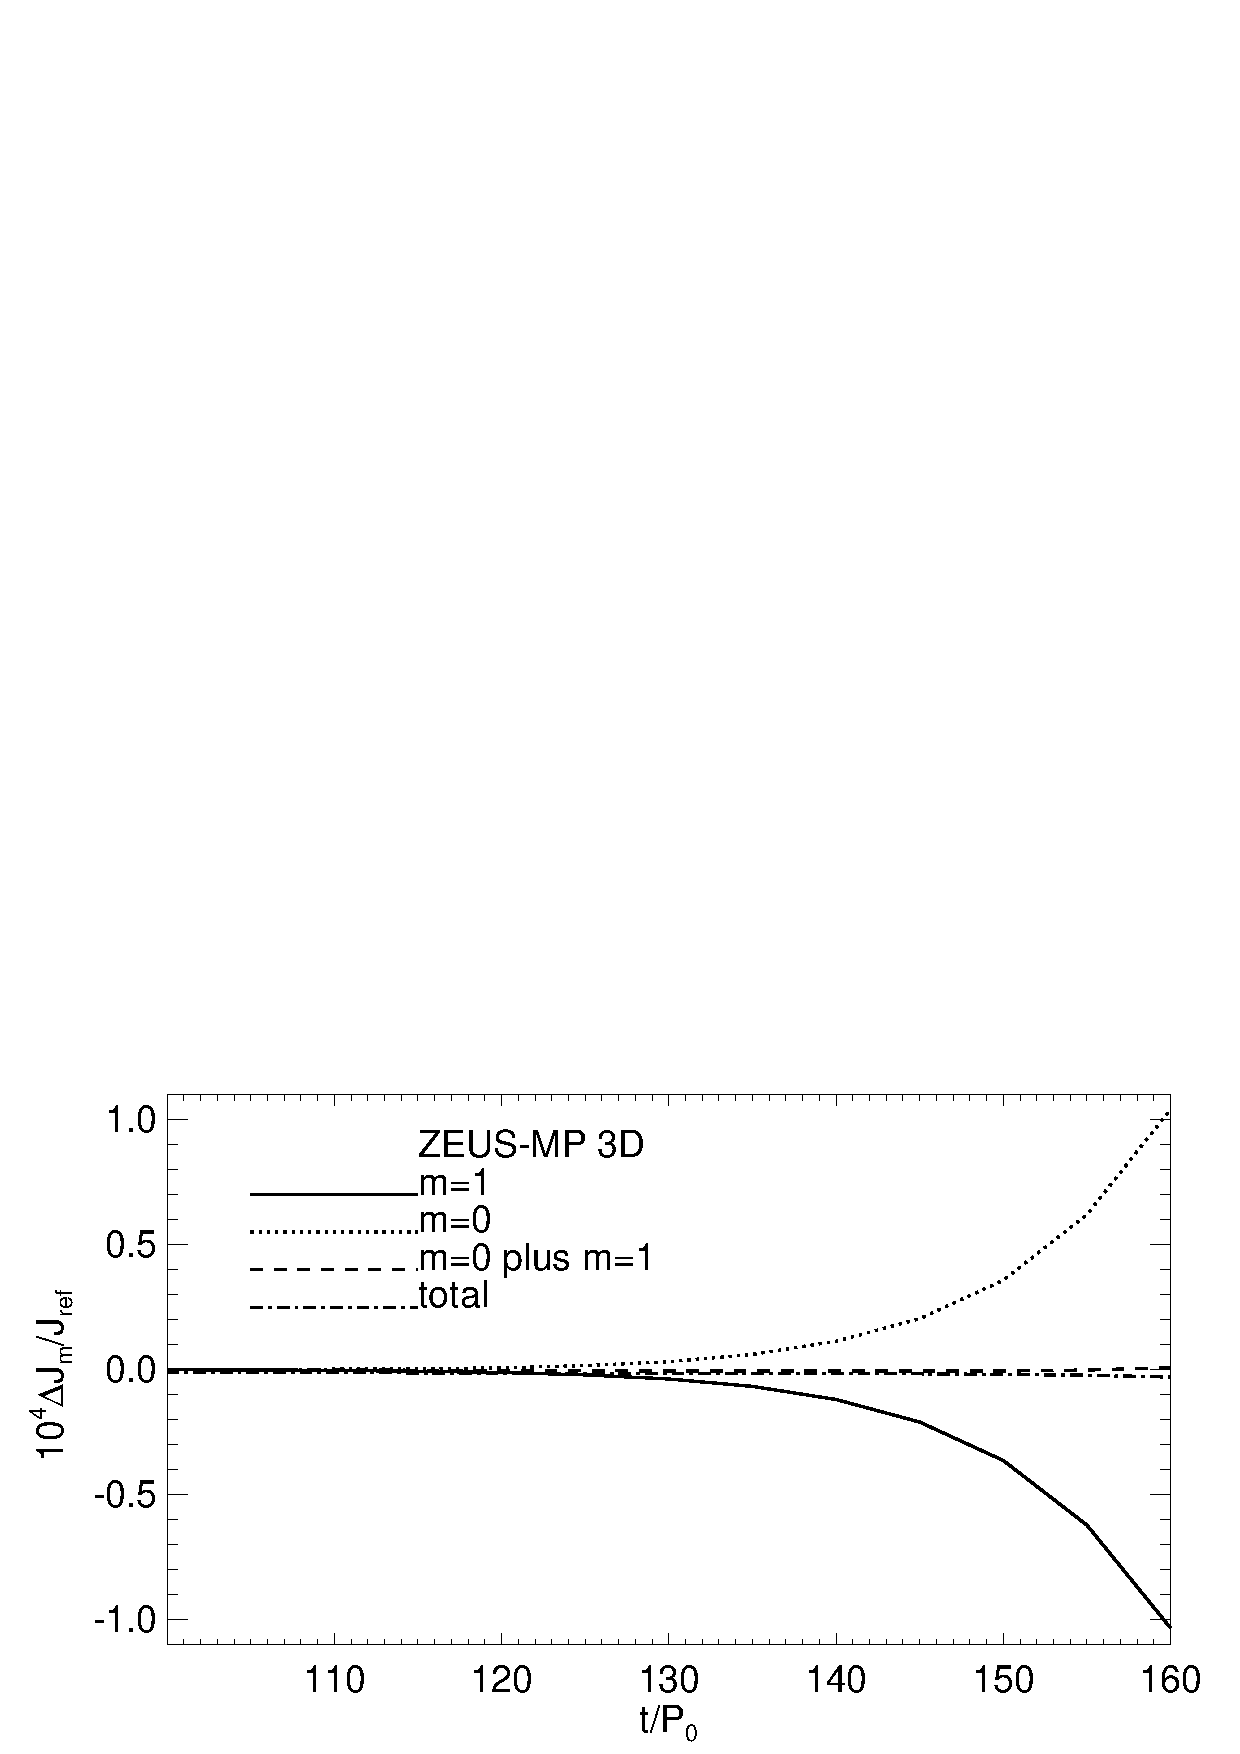
\includegraphics[scale=.41,clip=true,trim=0cm 1cm 0cm 0cm]{figures/nonaxi_evol_ang_zeus}
  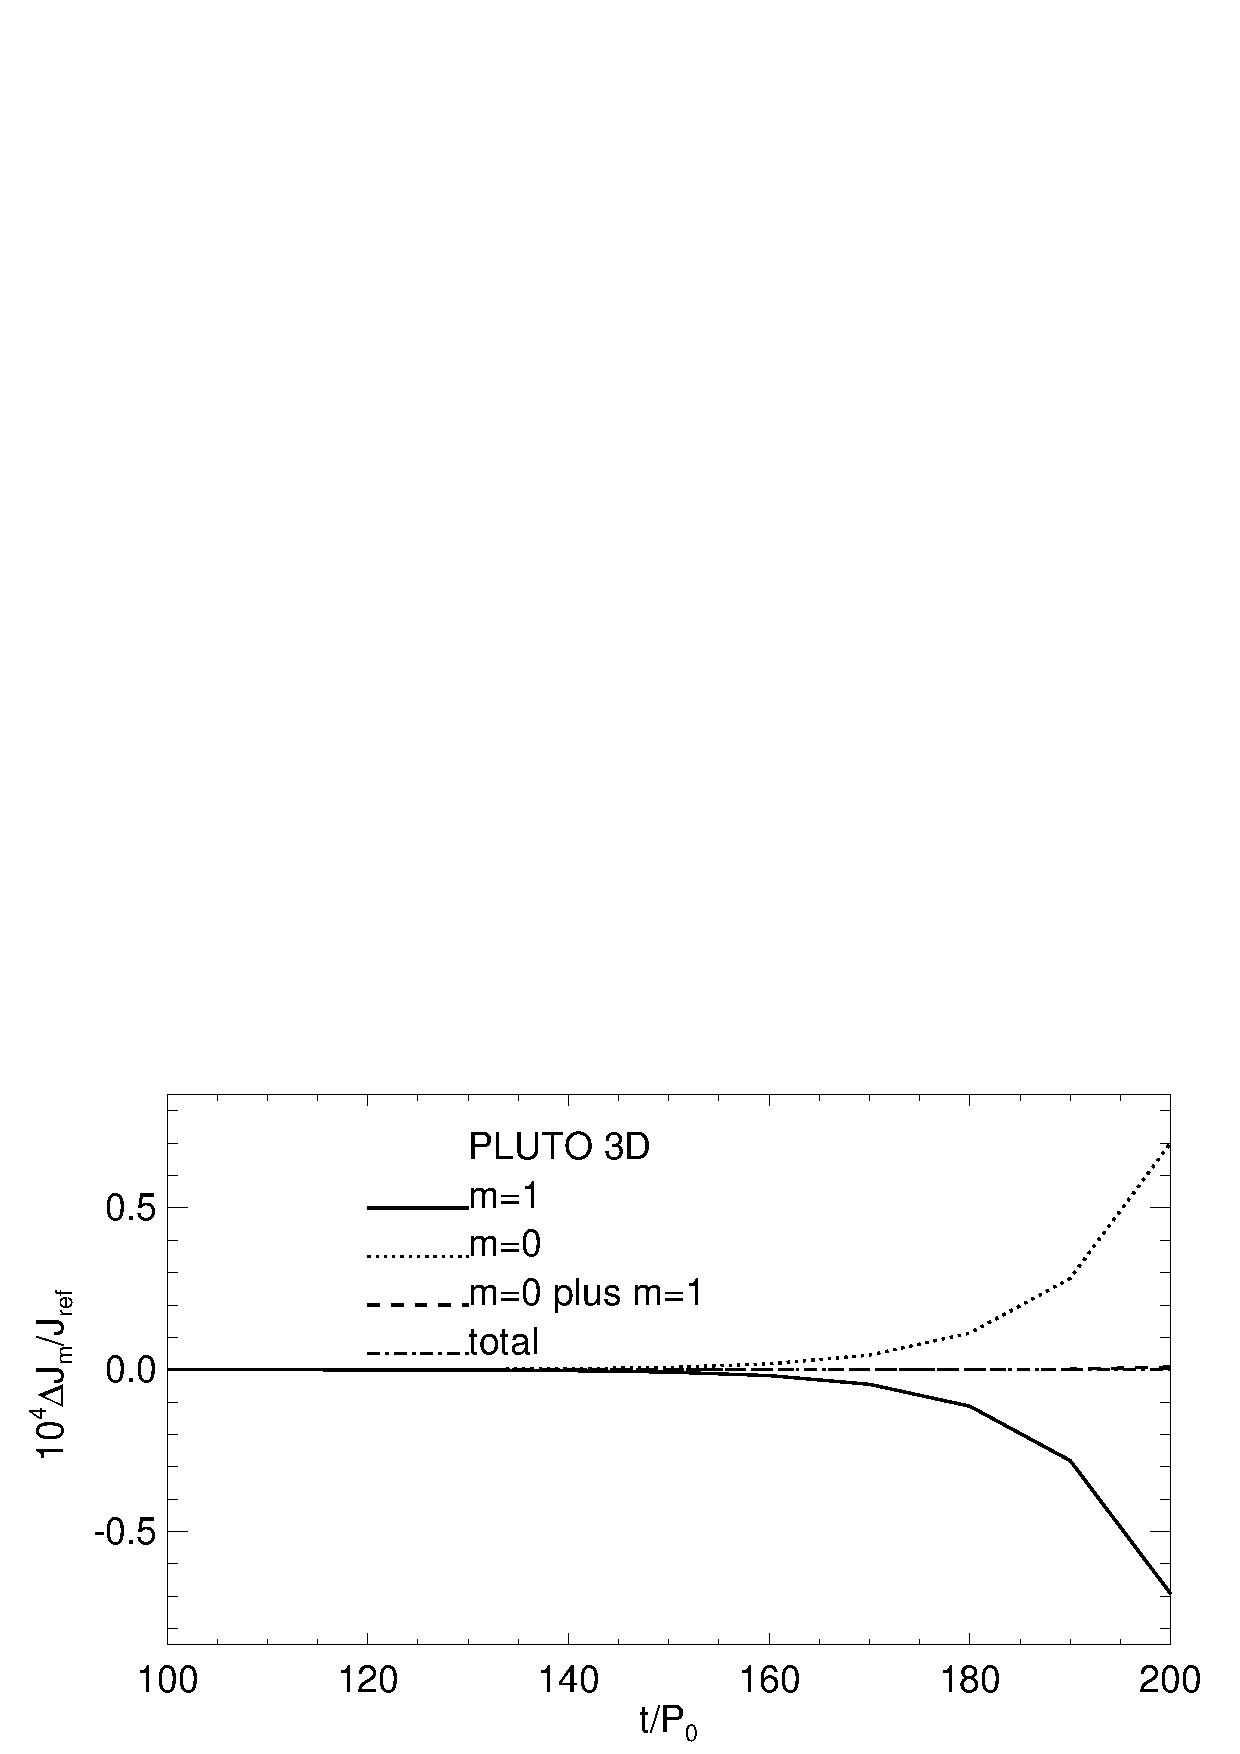
\includegraphics[scale=.41]{figures/nonaxi_evol_ang_pluto}
  \caption{Evolution of angular momentum components in the fiducial 3D 
    simulations. The perturbation
    relative to $t=100P_0$ is shown in units of the
    initial total angular momentum $J_\mathrm{ref}$.\label{3d_angmom}} 
\end{figure}   

